\section{Results and Analysis}
\label{Results}

All our networks give us about $93\%$ to $97.8\%$ classification accuracy on validation and test sets, but in this work we did not focus on getting a better classification accuracy.
Instead our major focus was to analyze the speedup obtained by parallelization, and the gigaflops of computation obtained for different batch sizes.

\begin{figure}[ht]
    \centering
    \begin{minipage}[t]{0.45\textwidth}
        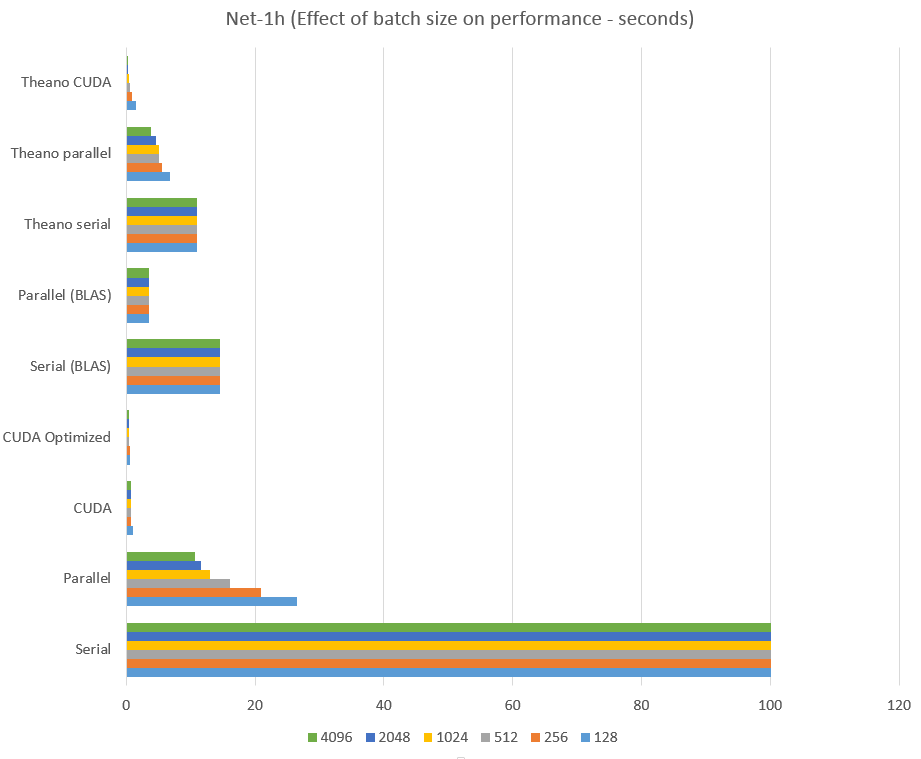
\includegraphics[width=\textwidth]{net1h_batch_secs.png}
        \caption{Time per epoch for Net-1h}
		\label{fig:nn1_time}
    \end{minipage}
    \begin{minipage}[t]{0.45\textwidth}   
		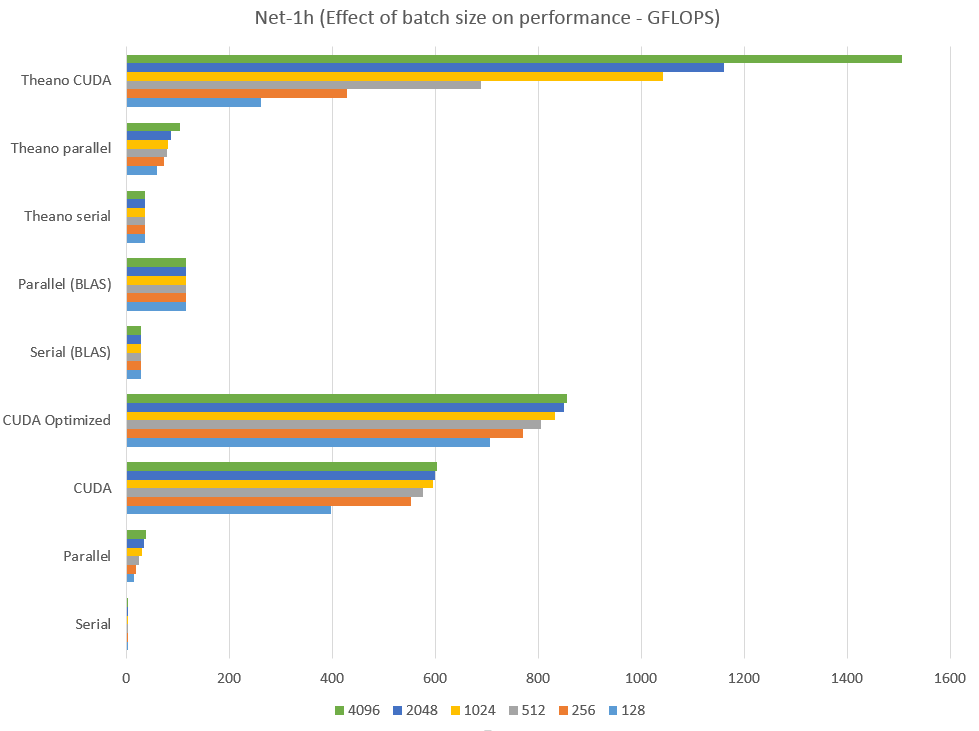
\includegraphics[width=\columnwidth]{net1h_batch_gflops.png}
		\caption{GFLOPS for Net-1h}
		\label{fig:nn1_gflops}
    \end{minipage}
\end{figure}

\begin{figure}[ht]
    \centering
    \begin{minipage}[t]{0.45\textwidth}
        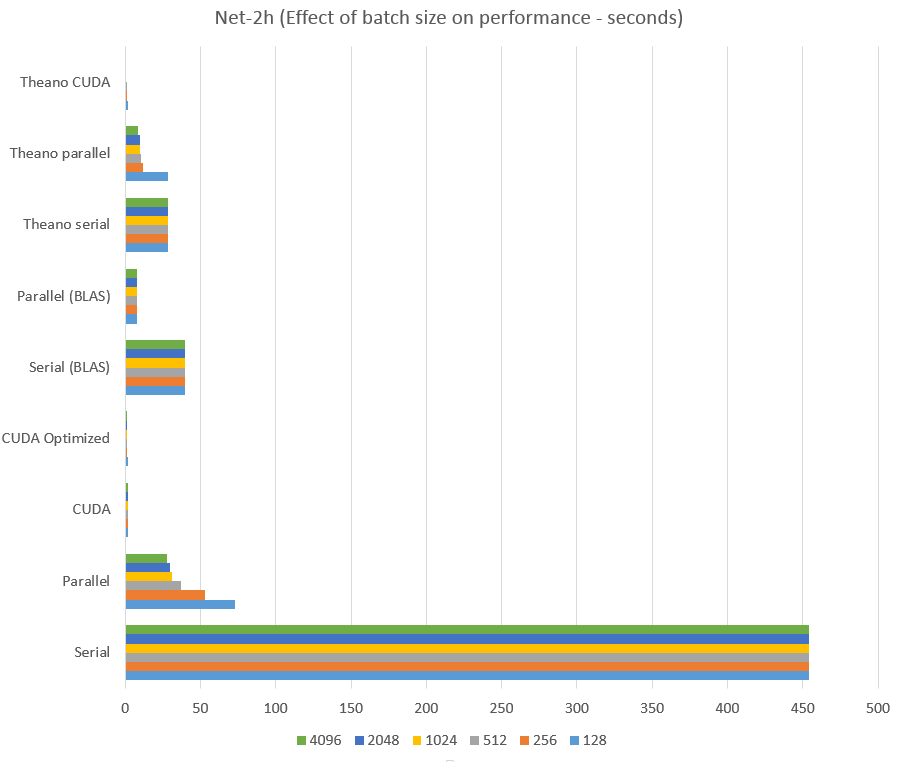
\includegraphics[width=\textwidth]{net2h_batch_secs.png}
        \caption{Time per epoch for Net-2h}
		\label{fig:nn2_time}
    \end{minipage}
    \begin{minipage}[t]{0.45\textwidth}   
		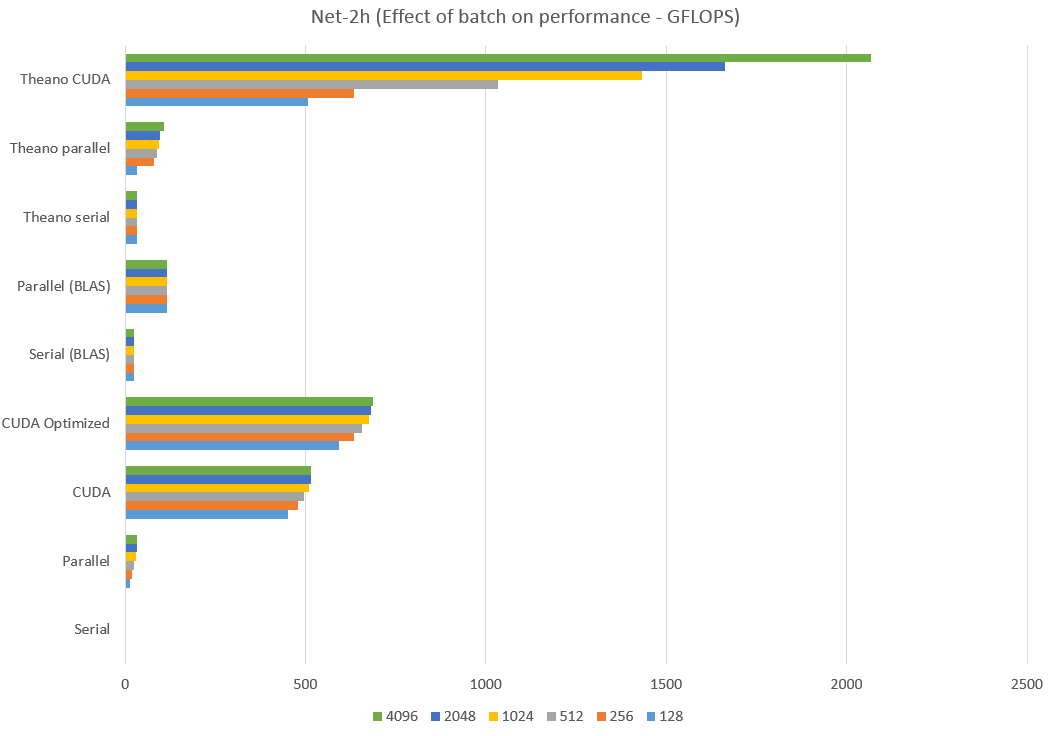
\includegraphics[width=\columnwidth]{net2h_batch_gflops.png}
		\caption{GFLOPS for Net-2h}
		\label{fig:nn2_gflops}
    \end{minipage}
\end{figure}

\begin{figure}[ht]
    \centering
    \begin{minipage}[t]{0.45\textwidth}
        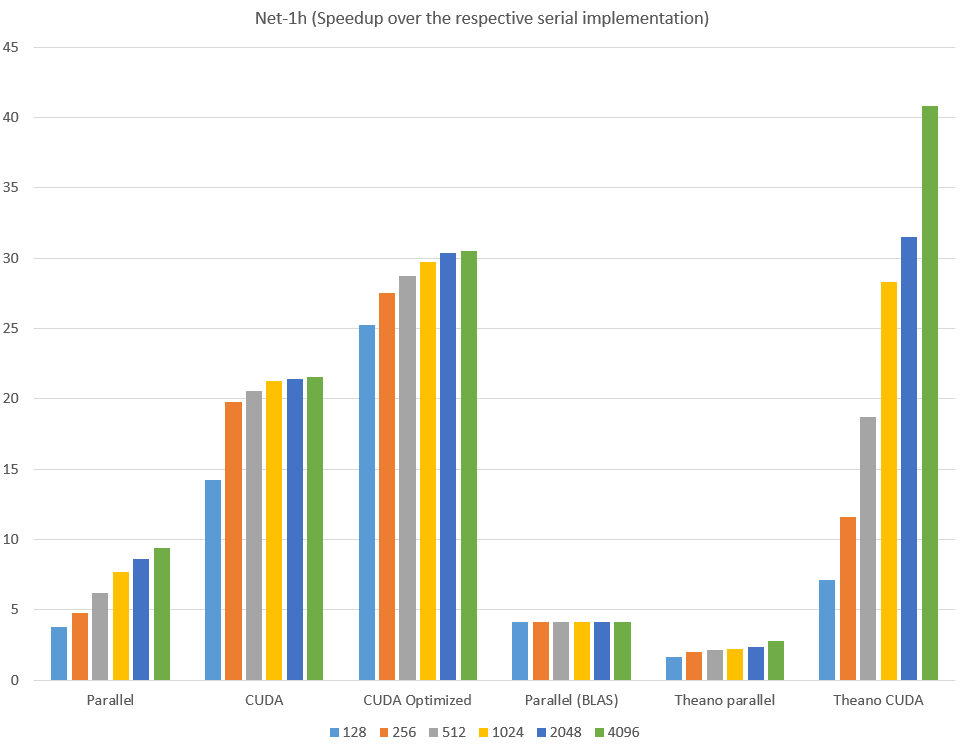
\includegraphics[width=\textwidth]{net1h_speedup.png}
        \caption{Speedup for Net-1h}
		\label{fig:nn1_speedup}
    \end{minipage}
    \begin{minipage}[t]{0.45\textwidth}   
		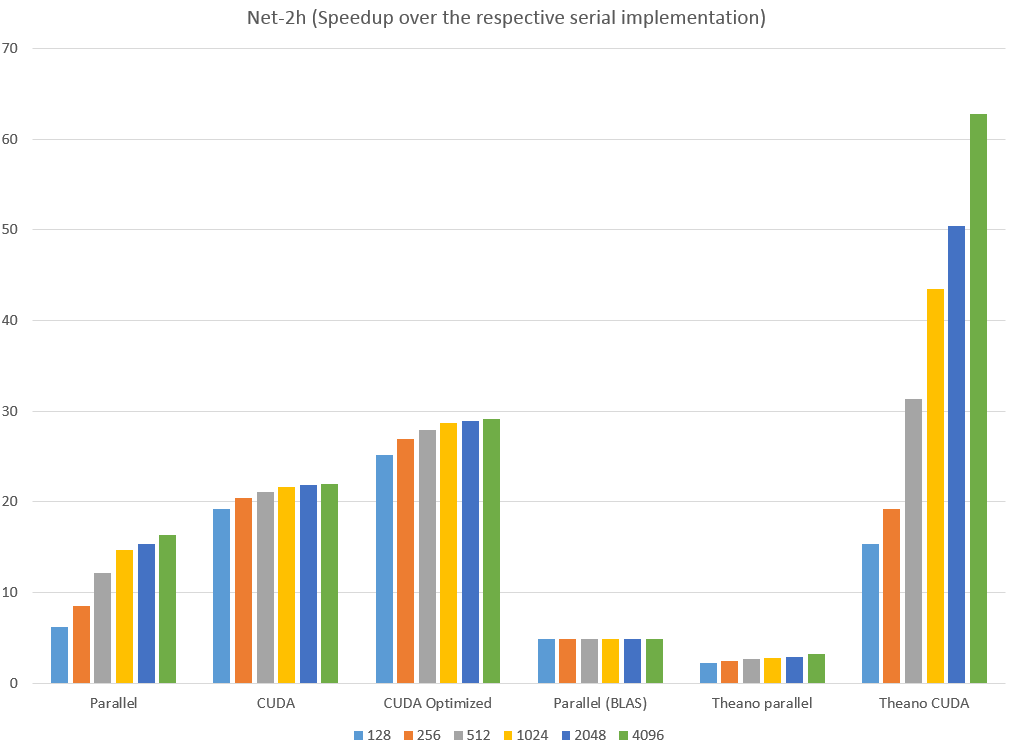
\includegraphics[width=\columnwidth]{net2h_speedup.png}
		\caption{Speedup for Net-2h}
		\label{fig:nn2_speedup}
    \end{minipage}
\end{figure}

Figures \ref{fig:nn1_time} and \ref{fig:nn2_time} show bar plots of the time per epoch (in seconds, called TPE henceforth) by all implementations as the batch size increases.
Figures \ref{fig:nn1_gflops} and \ref{fig:nn2_gflops} show the corresponding bar plots for amount of computation performed per epoch (in gigaflops, called GFLOPS henceforth).
The speedups (called SUP henceforth) obtained for Net-1h and Net-2h are shown in figures \ref{fig:nn1_speedup} and \ref{fig:nn2_speedup} respectively for various batch sizes.

The following points can be immediately observed from the figures:
\begin{itemize}
\item TPE and GFLOPS are constant for serial implementations regardless of batch sizes, which is to be expected because serial implementations access all data sequentially regardless of batch size.
\item TPE decreases and GFLOPS increases with increase in batch size for parallel and GPU implementations, which parallelize on training examples. This is expected since having more training examples in a batch reduce the thread creation overheads.
\item GPUs have a huge number of parallel cores and threads per core and hence they clearly dominate over the multicore parallel implementations at all values of batch sizes and network configurations.
\item BLAS parallel implementations do not exhibit a change in TPE or GFLOPS with increasing batch sizes, since they do not parallelize on minibatches.
\item Multicore Parallel and CUDA GPU implementations give an average speedup of approximately 10 and 25 respectively.
\item Theano serial and BLAS serial implementations are very efficient already and hence their parallel counterparts demonstrate a smaller speedup, although the parallel counterparts parallelizing on matrix computations clearly win over the parallel implementations parallelizing on training examples, in terms of GFLOPS.
\item Theano implementations (serial, parallel and GPU) use both types of parallelization and hence demonstrate lower TPE than all their corresponding counterparts for large batch sizes where efficiency of parallelized matrix operations matters a lot.
\item For smaller batch sizes around 128, our CUDA implementation dominates over Theano GPU because parallelization of matrix computations have a larger overhead at such scales with smaller matrix sizes. This is also reflected in Theano GPU's speedup, which grows extremely fast as batch size grows (figures \ref{fig:nn1_speedup} and \ref{fig:nn2_speedup}).
\end{itemize}

\textbf{BLAS} As Basic Linear Algebra Subprograms, BLAS has been a crucial workhorse in heavy numerical computing.
By replacing our self-built LINALGLIB with BLAS, we obtained hugely improved results.
Note that the execution time of BLAS doesn't depend on the number of threads because it parallelizes each Matrix-vector product and hence each thread executes different parts of the same example.
The serial implementation is still a bit slower than Theano but is faster than our previous implementation by about 10 times.

\textbf{GPU Bottlenecks} Ideally  the number of overheads (allocation/reduction) should be monotonically reduced by increasing the size of the batch.
However, our experiment results show that there are some performance bottlenecks. In our implementation, shared memory bank conflicts which reduce the parallelism when threads access the shared memory appear when the number of batches increase.
When the dimensions (i.e. number of neurons between layers) of the neural network are not perfect multiples of 32 then some threads do not participate in the computation which results in degraded parallelism.

Overall, we demonstrate that the parallel computation is significantly faster than the serial computation if we utilize multiple threads for processing many examples or do matrix-vector computations in parallel.
By dividing training datasets into larger mini batches, we are able to perform better due to reduced parallelization overheads.